\documentclass[12pt]{article}
\usepackage[utf8]{inputenc}
\usepackage[margin=2cm]{geometry}
\usepackage{listings}
\usepackage{graphicx}

\graphicspath{{imagens/}}

\begin{document}
\section{Introdução}
Tivemos como objetivo desse trabalho a elaboração e comparação de desempenho de quatro diferentes algoritmos de busca - sendo duas buscas cegas e duas buscas informadas.

\begin{itemize}
	\item As buscas cegas são:
	\begin{itemize}
		\item Busca em Profundidade;
		\item Busca em Largura.
	\end{itemize}
	\item As buscas informadas são:
	\begin{itemize}
		\item Best-first Search;
		\item A*.
	\end{itemize}
\end{itemize}

	Para isso foram utilizados tabuleiros tais como foram descritos na especificação do trabalho com uma origem, um destino e obstáculos distribuídos, os quais serão gerados a partir de um script de autoria própria.
	As métricas utilizadas para comparar os algoritmos são: tempo de execução, quantidade de casas no caminho encontrado, quantidade de casas analisadas (um vizinho no caso das buscas cegas e casas consideradas nas buscas informadas), quantidade de casas visitadas durante a execução e tamanho do caminho encontrado.
	O código foi desenvolvido em Python 3, sendo necessária a instalação do pacote celluloid (utilizado pelo grupo para gerar animações com a execução dos algoritmos). Para isso, basta executar o seguinte comando no terminal:

\begin{verbatim}
sudo pip3 install celluloid
\end{verbatim}

\section{Tabuleiros}
Foram criadas funções para criação, leitura e escrita de tabuleiros que serão usados no presente trabalho. Para a manipulação e visualização, mostrou-se mais fácil utilizar matrizes numéricas para representar os objetos sobre o tabuleiro, enquanto nos foi requisitado o uso de representação com caracteres para as casas na leitura e escrita dos tabuleiros. Desta forma, estabeleceu-se o código apresentado pela tabela \ref{codigo}, implementado no dicionário \verb|str2n| contido no arquivo \verb|utils.py|.

\begin{table}[h!]
	\label{codigo}
	\centering
	\begin{tabular}{c|c|c}
		Significado & Código de caracteres & Código numérico\\
		\hline
		Casa livre & * & 0\\
		Parede ou obstáculo & - & 4\\
		Casa objetivo & \$ & 3\\
		Casa de início da busca & \# & 2\\
		Marcações temporárias & (Nenhum) & \textless 1

	\end{tabular}
	\caption{Tabela de conversão entre os diferentes códigos utilizados no projeto.}
\end{table}

\subsection{Criação dos tabuleiros}
Criou-se algoritmo para a geração automática de tabuleiros, com suas paredes e os pontos de início e fim da busca. Visto que se deseja aparência semelhante à exposta na descrição do projeto (Figura \ref{tabuleiro_pedido}), não seria possível a geração completamente aleatória das paredes, e fez-se necessário desenvolver a estratégia descrita adiante.

\subsubsection{Visão geral}
 O processo de gerar tabuleiros é executado pelo script \texttt{gen\_boards.py}, mais especificamente e em seu mais alto nível pela função \verb|gen_board| implementada no referido \emph{script}, acontecendo da seguinte maneira:

\begin{enumerate}
	\item É criado um tabuleiro (matrix) em branco (preenchido com zeros), a partir das dimensões informadas com argumento;
	\item São sorteados dois pontos aleatoriamente para servirem de início e fim da busca. São sorteadas quantas vezes forem preciso até que tenham distância Manhattan entre si maior que um comprimento heuristicamente definido como a soma das dimensões do tabuleiro sobre 2;
	\item São construídas as paredes, como melhor explicado posteriormente.
\end{enumerate}

[código da função]

%Inicialmente criava-se um caminho aleatório para garantir que não houvesse
\subsubsection{Orquestração da contrução das paredes}

As peças mais importantes dese processo são as duas funções \verb|build_walls| e \verb|random_walk|, a primeira sendo de nível superior. O algoritmo de criação das paredes segue o seguinte raciocínio, coordenado pela \verb|build_walls|:

\begin{enumerate}
	\item Uma casa aleatória do tabuleiro (chamada \emph{seed} no código) é sorteada por meio da função \verb|seeds_gen|;
	\item É desenhada uma parede a partir dessa casa com a função random walk;
	\item O processo é repetido \verb|nseeds| vezes, um dos parâmetro sda função \verb|build_wals|, definido empiricamente por padrão como um décimo da área do tabuleiro.
\end{enumerate}

[código da função]


\subsubsection{Construção de cada parede}

A partir de cada semente (casa aleatória do tabuleiro) fornecida à função \verb|random_walk| pela função \verb|build_wals|, será traçada (ou pelo menos tentar-se-á traçar) uma nova parede. O papel da \verb|random_walk| é então "andar" pelas casas do tabuleiro marcando-do com o símbolo que designará aqueles quadrados como um novo obstáculo. A \verb|random_walk| pede como argumento duas funções essenciais, a \verb|end_func| e a \verb|turn_func|, que devem receber o comprimento do caminho traçado e retornar um valor booleao. O processo de traçado executado pela \verb|random_walk| é então esclarecido a seguir:

\begin{enumerate}
	\item A partir da posição inicial (argumento \verb|start|), verifica-se quais são os deslocametos unitários possíveis a partir \verb|start|, isto é, que não levarão a casas ocupadas por algum obstáculo, que levarão a casas marcadas com 0, e sorteia-se um desses "passos" (tuplas no formato (1,0), (-1, 1), (0, -1), etc.). Os passos podem ser restritos aos ortogonais (baixo, cima, direita, esquerda) definindo como \verb|True| o parâmetro \verb|orth|;
	\item Se não houver passo possível, a parede não é criada;
	\item Caso contrário desloca-se a posição para posição + passo e marca-se essa casa como parede (o número marcado é dado pelo argumento \verb|trail|). As outras casas do tabuleiro referentes aos outros passos possíveis não escolhidos são também marcadas com algum número menor que 1 (0.1 no caso), para que não sejam ocupadas em iterações posteriores e mantenham as paredes separadas entre si;
	\item Esse processo de deslocamento e marcação prossegue, avançando com o mesmo passo sorteado, na mesma direção, até que:
		\begin{enumerate}
			\item É encontrado um obstáculo (casa do tabuleiro com valor não nulo) à frente na direção escolhida atual;
			\item A função \verb|turn_func| retorne \verb|True|, caso em que a direção (passo) será sorteada novamente, ou;
			\item A função \verb|end_func| retorne \verb|True|, caso em que a criação da parede será finalizada.
		\end{enumerate}
\end{enumerate}

As funções \verb|end_func| e \verb|turn_func| são uma boa forma de controlar a dinâmica da criação de paredes. Se esses argumentos da função \verb|random_walk| são providos a ela como \verb|floats| entre 0 e 1, a \verb|random_walk| os substitui por funções que retornam \verb|True| com a probabilidade representada pelos \verb|floats| fornecidos.\\

Outra possibilidade criada, é fornecer um inteiro como argumento \verb|len| para a \verb|random_walk|, caso em que \verb|end_func| se torna função que retorna \verb|True| se a distância traçada for maior que o inteiro fornecido. Nesse caso, o inteiro representaria um comprimento máximo para a parede, de forma que ela seria finalizada por colisão com uma casa não vazia ou por atingir esse comprimento máximo.

Para os experimentos são usadas \verb|turn_func = 0.2| e \verb|end_func = 0|, de forma que há sempre um quinto de probabilidade de virar, e a parede será desenhada até que se encontre um obstáculo.

\begin{figure}[h!]
	\centering
	\label{fig:trapezoidal}
	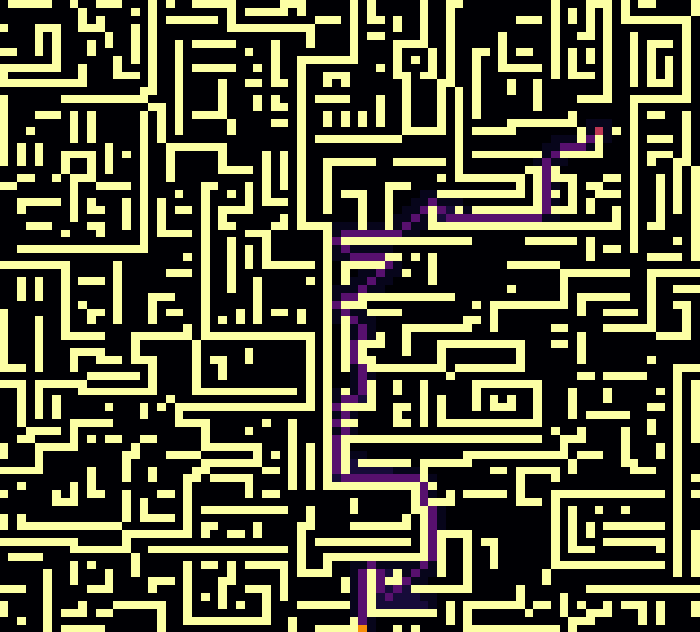
\includegraphics[width=.7\textwidth]{80x80}
	\caption{Exemplo de tabuleiro 80x80 criado com o algoritmo descrito. A casa vermelha é a posição de início da busca, e a laranja é a casa-objetivo.}
\end{figure}


\section{Algoritmos de busca}
Todos os algoritmos de busca possuem o mesmo cabeçalho:

\begin{lstlisting}[language=Python]
def search(board: list, origin: tuple,
	target: tuple, camera: Camera = None) -> list:
\end{lstlisting}

em que \verb|board| é o tabuleiro, \verb|origin| é a tupla da casa de início, \verb|target| é a tupla da casa de destino e \verb|camera| é utilizada somente na criação de imagens GIF para visualização do caminho tomado pelo algoritmo.

\subsection{Busca cega}
Nessa modalidade de busca, o algoritmo não faz uso de nenhuma informação sobrea localização de casa-alvo. Os tipos implementados são descritos a seguir.

\subsubsection{Busca em profundidade}
A busca em profundidade está na função search no arquivo \verb|depth_first_search.py|. Inicialmente criamos uma função para que retorne o caminho encontrado pelo algoritmo.\\

As variáveis \verb|visited| e \verb|processed| são, respectivamente, um deque e um set, estruturas otimizadas para o nosso uso (deque é otimizada para operações de inserção/deleção do início ou final da lista e set para a busca de um elemento). Inicialmente inserimos a tupla da \verb|origem| em \verb|visited| e \verb|processed|, em seguida iniciamos um loop que ocorre enquanto houver tuplas em \verb|visited| (ou até chegar no destino) e a variável pos recebe a tupla que está no início de \verb|visited|. Essa posição no tabuleiro é marcada como visitada.\\

Após isso verificamos os vizinhos de pos utilizando a função \verb|available_moves| que retorna apenas as casas ainda não processadas, elas são adicionados no início de \verb|visited| (serão os próximas casas processadas) e marcamos que pos é a casa antecessora delas a fim de obtermos o caminho após a execução do algoritmo.\\

Depois de explorar todos os vizinhos, se quisermos criar um gif é “tirada uma foto” do tabuleiro e reinicia-se o processo com pos recebendo a tupla no início de \verb|visited|.
Se não for encontrado um caminho a função retorna \verb|None|.


\subsubsection{Busca em largura}
A função para realizar a busca em largura é totalmente análoga a de busca em profundidade, no entanto ao invés de adicionar os vizinhos de pos no início de visited, eles são adicionados no final.


\subsection{Busca informada}
Nos algoritmos de busca informada, utiliza-se o conhecimento das coordenadas do alvo para guiar a procura. Contudo, a presença e localização dos obstáculos não é conhecida, e faz-se necessário que o algoritmo determine os melhores caminhos alternativos de desvio.\\

Como nas buscas cegas, cria-se uma lista de casas a serem visitadas conforme se explora o tabuleiro. Contudo, a diferença essencial é a forma como os elementos são retirados dessa lista: A cada casa com coordenadas \verb|pos| que se pretende adicionar à lista, utiliza-se uma função chamada \verb|f(pos)|, que, em posse do conhecimento da posição da casa-objetivo, fornece um valor peso para a nova casa explorada. Esses pesos são interpretados como o quanto será favorável explorar aquele casa ou não, de forma que ao ser inserida a casa na lista, cria-se naturalmente uma fila de prioridades em função da ordem desses valores peso.\\

Essa função \verb|f(pos)| ainda se desdobra em dois termos:

\begin{verbatim}
f(pos) = g(pos) + h(pos),
\end{verbatim}

sendo que \verb|g(pos)| retorna a distância de \verb|pos| até a casa inicial, isto é, o quanto teríamos nos deslocado durante a busca desde o início caso estivéssemos em \verb|pos|; e \verb|f(pos)| retorna uma estimativa da distância entre \verb|pos| e o alvo.\\

O caso mais geral desse tipo de busca, que abrange todas as buscas que usam a função \verb|f(pos)| como descrito é a busca A* (pronunciada "A estrela"). No caso específico em que \verb|g(pos)| seja 0, o algoritmo é chamado, \emph{algoritmo de Dijkstra}, não utilizado no presente trabalho. Se, por sua vez, \verb|g(pos)| seja definida como 0, o algoritmo é chamado busca \emph{best-first}.\\

Sobre o cálculo das distâncias, além da norma euclideana mais canonicamente utilizada em problemas do tipo, faz-se experimentações com uma função norma diferentemente pensada, aqui chamada \emph{distância trapezoidal}, justamente por se comportar da forma apresentada na figura \ref{fig:trapezoidal}.

\begin{figure}[h!]
	\centering
	\label{fig:trapezoidal}
	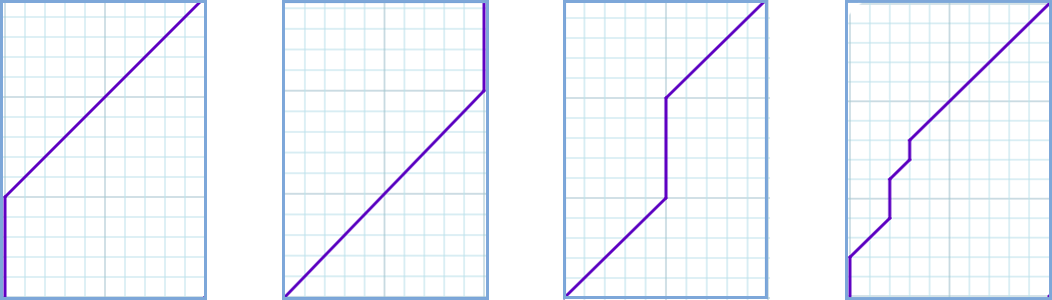
\includegraphics[width=.9\textwidth]{trapezoidal}
	\caption{Várias representações da mesma distância trapezoidal entre pontos em vértices opostos do retângulo.}
\end{figure}

Dada sua representação, se os pontos que se distam formam um retângulo de lados \(a\) e \(b\) e assumindo \(a > b\) sem perda de generalidade, temos que a norma trapezoidal será dada por \(\sqrt{2}a + (a - b)\), ou em código:\\

\begin{lstlisting}[language=Python]
def trapezoidal_dist(pos: tuple, target: tuple) -> float:
    """ Distancia trapezoidal de pos a target """
    if pos not in trapezoidal_dist.values:
        a = abs(pos[0] - target[0])
        b = abs(pos[1] - target[1])
        d = abs(a-b)
        trapezoidal_dist.values[pos] = sqrt(2) * min(a, b) + d
    return trapezoidal_dist.values[pos]
\end{lstlisting}

Em que se armazena dinamicamente os resultados para futuras consultas.\\

É possível provar, embora fuja do escopo do presente trabalho que, dadas as restrições de movimento impostas, a distância trapezoidal é a mínima distância percorrida pelos algoritmos de busca, de forma a fazer com que a heurística assuma o máximo valor ainda ótimista para as trajétorias de busca, favorecendo tempo de processamento sem deixar de garantir que o mehor caminho seja retornado na busca A*.

\subsubsection{Busca \emph{best-first}}

Esse algoritmo de busca é implementado no arquivo \verb|best_first.py|, e, como antes dito, é caracterizada pelo uso de heurística que considera somente a distância estimada ao alvo a partir da casa sendo visitada. Assim sendo, não há garantia de retorno do caminho ótimo, pois não se leva em conta o peso do caminho da posição inicial à casa visitada.\\

A função \verb|search| no arquivo, responsável por executar a busca, utiliza um set com as casas visitadas, para se certificar de que não entre em loop visitando a mesma casa mais de uma vez.\\

A lista \verb|queue| é justamente a responsável por guardar os camihos percorridos. Cada vez que uma casa é visitada, ela é substituída pela concatenação entre ela e seus filhos, de forma que cada item de \verb|queue| seja uma tupla com o caminho todo percorrido até uma determinada casa e o valor de peso retornado pela função heurística. As funções \verb|heappop| e \verb|heappush| do módulo \verb|heap| são responsáveis por inserir e retirar os caminhos da lista mantendo sua ordem de prioridades.\\

A identificação de casas filhas disponíveis é feita pela função \verb|available_moves|, contida no arquivo \verb|utils.py|.

\subsubsection{Busca A*}
Como antes mencionado, a busca por novas células através do algoritmo A* é feita utilizando dois cálculos: uma função \verb|g| que determina o custo do caminho da origem até a posição atual, e outra função \verb|h| (heurística) que determina um custo estimado otimista do caminho da posição atual até o destino. Estamos interessados em uma função \verb|f| tal que \verb|f = g + h|.\\

O cálculo de g está implementado no arquivo \verb|a_star.py|, na função \verb|calc_g(pos1, pos2)|, sendo \verb|pos2| a posição que se deseja explorar e \verb|pos1| o nó pai de \verb|pos2| no tabuleiro. Inicialmente, a função \verb|calc_g()| determina se \verb|pos1| e \verb|pos2| diferem em apenas uma dimensão ou em ambas (variável \verb|dist|): caso \verb|dist| seja igual a 1 sabemos que o passo foi dado em uma mesma dimensão, portanto o peso do passo será igual a 1; caso contrário (\verb|dist| igual a 2) sabemos que o passo foi dado em uma diagonal, então o peso do passo será igual a \(\sqrt{2}\). Por fim, obtemos o valor de \verb|g| para \verb|pos2| somando o valor anterior com o valor de \verb|g| já calculado anteriormente para \verb|pos1|, e armazenamos esse valor em uma estrutura de dicionário caso já não o possua ou o novo valor seja menor que o anterior.\\

A cálculo de \verb|h| pode ser obtido através de duas funções (heurísticas) diferentes, ambas implementadas no arquivo \verb|util.py|: distância euclidiana (função \verb|euclidian_dist(pos, target)|) e distância trapezoidal (função \verb|trapezoidal_dist(pos, target)|). \verb|euclidian_dist| é a distância euclidiana (linha reta) entre \verb|pos| e \verb|target|, \verb|trapezoidal_dist| simula a distância que seria de fato percorrida caso não houvessem obstáculos, portanto segue o formato de um trapézio. Por conta disso, a primeira função é mais otimista do que a segunda e, portanto, espera-se que a primeira seja mais lenta.\\

A busca A* está implementada no arquivo \verb|a_star.py|, na função \verb|search(board, origin, target)|, onde \verb|board| é o tabuleiro (labirinto), \verb|origin| é a posição inicial e \verb|target| é a posição destino. Dentro dessa função está declarada a função \verb|calc_path(parents)|, cujo objetivo é calcular o caminho percorrido desde \verb|target| até \verb|origin|, utilizando o dicionário \verb|parents| que foi gerado durante a busca e representa a posição pai de cada posição visitada.\\

Na busca em si utilizamos 5 estruturas de dados: \verb|open_list| é uma fila de prioridades que guarda as posições que foram analisadas porém ainda não foram totalmente processadas (ou seja, seus filhos não foram analisados), o parâmetro de ordenação da fila de prioridades é o valor de \verb|f| de cada posição; \verb|closed_list| é uma estrutura do tipo set que guarda as posições já totalmente processadas, ele é utilizado para verificar se a próxima posição a ser analisada ainda não foi processada (caso tenha sido, essa posição é ignorada), o tipo set foi utilizado para otimizar a busca e inserção, cujas complexidades são O(1) (constantes); \verb|parents| é um dicionário (par chave-valor) onde as chaves são posições do tabuleiro e o valor é o respectivo pai da posição na chave; \verb|calc_g.values| é um dicionário pertencente à função \verb|calc_g| e guarda os cálculos do menor \verb|g| para cada posição \verb|pos2| do tabuleiro, partindo de \verb|pos1|; \verb|trapezoidal_dist.values| pertence à função \verb|trapezoidal_dist| e guarda os cálculos da heurística \verb|h| em distância trapezoidal para cada posição pos do tabuleiro até o destino. No loop principal da busca, o algoritmo checa de \verb|open_list| está vazio, retira a próxima posição de \verb|open_list| (com menor valor de f), checa se a posição é o destino (caso for, encerra a busca e calcula o caminho),
\end{document}
